% Definiciones y constantes de estilo
% Clase del documento
\documentclass[a4paper,12pt,twoside,openright,titlepage]{book}

%
% Paquetes necesarios
%

% Símbolo del euro
\usepackage{eurosym}
% Codificación UTF8
\usepackage[utf8]{inputenc}
% Caracteres del español
\usepackage[spanish]{babel}
% Código, algoritmos, etc.
\usepackage{listings}
% Definición de colores
\usepackage{color}
% Extensión del paquete color
\usepackage[table,xcdraw]{xcolor}
% Márgenes
\usepackage{anysize}
% Cabecera y pie de página
\usepackage{fancyhdr}
% Estilo título capítulos
\usepackage{quotchap}
% Algoritmos (expresarlos mejor)
\usepackage{algorithmic}
% Citas mejoradas
\usepackage{cite}
% Títulos de secciones
\usepackage{titlesec}
% Fórmulas matemáticas
\usepackage[cmex10]{amsmath}
% Enumeraciones
\usepackage{enumerate}
% Páginas en blanco
\usepackage{emptypage}
% Separación entre cajas
\usepackage{float}
% Imágenes
\usepackage[pdftex]{graphicx}
% Mejora de las tablas
\usepackage{array}
% Mejora de los símbolos matemáticos
\usepackage{mdwmath}
% Separar figuras en subfiguras
\usepackage[caption=false,font=footnotesize]{subfig}
% Incluir pdfs externos
\usepackage{pdfpages}
% Mejoras sobre las cajas
\usepackage{fancybox}
% Apéndices
\usepackage{appendix}
% Marcadores (para el pdf)
\usepackage{bookmark}
% Estilo de enumeraciones
\usepackage{enumitem}
% Espacio entre líneas y párrafos
\usepackage{setspace}
% Glosario/Acrónimos
\usepackage[acronym]{glossaries}
% Fuentes
\usepackage[T1]{fontenc}

% Enlaces
\hypersetup{hidelinks,pageanchor=false,colorlinks,citecolor=Fuchsia,urlcolor=black,linkcolor=Cerulean}

% Fix warning
\setlength{\headheight}{16pt}

% Euro (€)
\DeclareUnicodeCharacter{20AC}{\euro}

% Estilo de la bibliografía
\bibliographystyle{IEEEtran}
\addto{\captionsspanish}{\renewcommand{\bibname}{Referencias}}

% Inclusión de gráficos
\graphicspath{{./graphics/}}

% Extensiones de gráficos
\DeclareGraphicsExtensions{.pdf,.jpeg,.jpg,.png}

% Definiciones de colores (para hidelinks)
\definecolor{LightCyan}{rgb}{0,0,0}
\definecolor{Cerulean}{rgb}{0,0,0}
\definecolor{Fuchsia}{rgb}{0,0,0}

% Keywords (español e inglés)
\def\keywordsEn{\vspace{.5em}
{\textbf{\textit{Key words ---}}\,\relax%
}}
\def\endkeywordsEn{\par}

\def\keywordsEs{\vspace{.5em}
{\textbf{\textit{Palabras clave ---}}\,\relax%
}}
\def\endkeywordsEs{\par}


% Abstract (español e inglés)
\def\abstractEs{\vspace{.5em}
{\textbf{\textit{Resumen ---}}\,\relax%
}}
\def\endabstractEs{\par}

\def\abstractEn{\vspace{.5em}
{\textbf{\textit{Abstract ---}}\,\relax%
}}
\def\endabstractEn{\par}

% Estilo páginas de capítulos
\fancypagestyle{plain}{
\fancyhf{}
\fancyfoot[CO]{\footnotesize\emph{\nombretrabajo}}
\fancyfoot[RO]{\thepage}
\renewcommand{\footrulewidth}{.6pt}
\renewcommand{\headrulewidth}{0.0pt}
}

% Estilo resto de páginas
\pagestyle{fancy}

% Estilo páginas impares
\fancyfoot[CO]{\footnotesize\emph{\nombretrabajo}}
\fancyfoot[RO]{\thepage}
\rhead[]{\leftmark}

% Estilo páginas pares
\fancyfoot[CE]{\emph{\pieparcen}}
\fancyfoot[LE]{\thepage}
\fancyfoot[RE]{\pieparizq}
\lhead[\leftmark]{}

% Guía del pie de página
\renewcommand{\footrulewidth}{.6pt}

% Nombre de los bloques de código
\renewcommand{\lstlistingname}{Código}

% Estilo de los lstlistings
\lstset{
    frame=tb,
    breaklines=true,
    postbreak=\raisebox{0ex}[0ex][0ex]{\ensuremath{\color{gray}\hookrightarrow\space}}
}

% Definiciones de funciones para los títulos
\newlength\salto
\setlength{\salto}{3.5ex plus 1ex minus .2ex}
\newlength\resalto
\setlength{\resalto}{2.3ex plus.2ex}

% Estilo de los acrónimos
\renewcommand{\acronymname}{Glosario}
\renewcommand{\glossaryname}{Glosario}
\pretolerance=2000
\tolerance=3000
\renewcommand{\glsnamefont}[1]{\makefirstuc{#1}}

% Pie de tabla
\addto\captionsspanish{
\def\tablename{Tabla}
\def\listtablename{\'Indice de tablas}
}

% Traducir appendix/appendices
\renewcommand\appendixtocname{Apéndices}
\renewcommand\appendixpagename{Apéndices}

% Comando code (lstlisting sin cambio de página)
\lstnewenvironment{code}[1][]%
  { \noindent\minipage{0.935\linewidth}\medskip
    \vspace{5mm}
    \lstset{basicstyle=\ttfamily\footnotesize,#1}}
  {\endminipage}

% Estilo JSON en listing
\colorlet{punct}{red!60!black}
\definecolor{background}{HTML}{EEEEEE}
\definecolor{delim}{RGB}{20,105,176}
\colorlet{numb}{magenta!60!black}
\lstdefinelanguage{json}{
    basicstyle=\normalfont\ttfamily,
    stepnumber=1,
    numbersep=8pt,
    showstringspaces=false,
    breaklines=true,
    backgroundcolor=\color{background},
    literate=
     *{0}{{{\color{numb}0}}}{1}
      {1}{{{\color{numb}1}}}{1}
      {2}{{{\color{numb}2}}}{1}
      {3}{{{\color{numb}3}}}{1}
      {4}{{{\color{numb}4}}}{1}
      {5}{{{\color{numb}5}}}{1}
      {6}{{{\color{numb}6}}}{1}
      {7}{{{\color{numb}7}}}{1}
      {8}{{{\color{numb}8}}}{1}
      {9}{{{\color{numb}9}}}{1}
      {:}{{{\color{punct}{:}}}}{1}
      {,}{{{\color{punct}{,}}}}{1}
      {\{}{{{\color{delim}{\{}}}}{1}
      {\}}{{{\color{delim}{\}}}}}{1}
      {[}{{{\color{delim}{[}}}}{1}
      {]}{{{\color{delim}{]}}}}{1},
}

% Definiciones de comandos
\newcommand{\nombreautor}{Juan Sidrach de Cardona Mora}
\newcommand{\nombretutor}{Dr. Sergio López-Buedo}
\newcommand{\nombretrabajo}{Interfaz web para la gestión de sondas de red de altas prestaciones}
\newcommand{\fecha}{Junio 2014}
\newcommand{\grado}{Doble Grado en Ingeniería Informática y Matemáticas}
\newcommand{\grupoInvestigacion}{High Performance Computing and Networking Research Group}
\newcommand{\departamento}{Dpto. de Tecnología Electrónica y de las Comunicaciones}
\newcommand{\facultad}{Escuela Politécnica Superior}
\newcommand{\universidad}{Universidad Autónoma de Madrid}
\newcommand{\pieparizq}{\href{https://github.com/JSidrach/NetWatcher}{\scriptsize{github.com/JSidrach/NetWatcher}}}
\newcommand{\pieparcen}{Trabajo de Fin de Grado}
\newcommand{\logoizq}{Logo_EPS}
\newcommand{\logoder}{Logo_UAM}
\newcommand{\correo}{***REMOVED***}

% Glosario y acrónimos
\makeglossaries
% Acrónimos

% TODO: Añadir aquí los acrónimos
% Ejemplo de acrónimo
\newacronym{FPGA}{FPGA}{Field-Programmable Gate Array}
\newacronym{IFG}{IFG}{InterFrame Gap (TODO)}

% Glosario

% TODO: Añadir aquí las definiciones del glosario
% Ejemplo de glosario
\newglossaryentry{bitstream}{name={bitstream},description={En este contexto se refiere al binario que configura el Hardware de la FPGA}}
\newglossaryentry{traza}{name={traza},plural={trazas},description={TODO: traza}}
\newglossaryentry{simple}{name={simple},description={TODO: simple}}
\newglossaryentry{pcap}{name={pcap},description={TODO: pcap}}


% Inicio del documento
\begin{document}

% Elección del idioma (español)
\selectlanguage{spanish}

%
% Portada
%
\pagenumbering{gobble}
\include{portada}

%
% Agradecimientos
%
\pagenumbering{Roman}
\setcounter{page}{0}
\include{src/agradecimientos}  

%
% Resumen
%
\include{src/resumen}

%
% Glosario
%
\printglossary[title=Glosario,toctitle=Glosario]
\printglossary[title=Acrónimos,toctitle=Acrónimos,type=\acronymtype]

%
% Tabla de contenidos
%
\tableofcontents
\listoftables
\listoffigures
\cleardoublepage

% Estilo de párrafo de los capítulos
\setlength{\parskip}{0.75em}
\renewcommand{\baselinestretch}{1.25}
% Interlineado
\spacing{1.3}
% Numeración contenido
\pagenumbering{arabic}
\setcounter{page}{1}

%
% Capítulos
%
\chapter{Introducción}

TODO: Introducción del trabajo
interfaz web para la gestión de sondas de red de altas prestaciones. HPCN. Ámbito, motivación y objetivos de este Trabajo de Fin de Grado, seguidos de una explicación sobre la estructura del documento.

Una sonda de red es simplemente un dispositivo capaz de capturar tráfico de red (sonda
pasiva) o de inyectarlo (sonda activa). Este dispositivo puede ser algo tan sencillo
como un ordenador convencional, en el que se ha instalado una tarjeta Ethernet
estándar o una tarjeta a medida basada en FPGA (ver la propuesta de proyecto
“Sistema basado en FPGA para la captura de tráfico en redes multigigabit Ethernet”).
Este ordenador típicamente correrá un sistema operativo Linux/GNU, y se habrán
instalado unos drivers especiales para poder acceder lo más eficientemente a la tarjeta
de red. Lo habitual es manejar la sonda desde línea de comandos. En este proyecto se
propone hacer una interfaz de usuario mucho más amigable, basada en web. En la
sonda correrá un servidor web, que mostrará una página con la que se podrá configurar
y manejar todos los aspectos de la sonda (capturar tráfico, reproducirlo, estado de la
sonda). Todas estas operaciones se corresponden con ejecutar programas de línea de
comandos, por lo que en resumidas cuentas este proyecto consiste en hacer un frontend
web para una interfaz de línea de comandos.
La interfaz web no solo tendrá una sección de controles para manejar la sonda, sino que
también mostrará su estado de una manera gráfica (medidores de nivel, etc.) y dibujará
alguna gráfica sencilla (bytes recibidos vs. tiempo, etc.)


\section{\'Ambito}

Trabajo de Fin de Grado

 sondas de red de altas prestaciones

grupo de investigación \textit{High Performance Computing and Networking}. 

TODO: Ámbito del trabajo


\section{Motivación}

Necesaria simplificación gestión de sondas de red de altas prestaciones por medio de una interfaz gráfica

ampliar la funcionalidad ofreciendo monitorización 
TODO: Motivación del trabajo


\section{Objetivos}

Este Trabajo de Fin de Grado tiene los siguientes objetivos principales:

\begin{itemize}
  \item Desarrollar una interfaz web que permita la gestión de sondas de red de altas prestaciones de manera intuitiva y sencilla.
  Desarrollar una interfaz web que permita la gestión de sondas de red de altas prestaciones de manera intuitiva y sencilla.
  Desarrollar una interfaz web que permita la gestión de sondas de red de altas prestaciones de manera intuitiva y sencilla.

  \item Monitorizar el estado del servidor al que está conectada una sonda de red de altas prestaciones.
Desarrollar una interfaz web que permita la gestión de sondas de red de altas prestaciones de manera intuitiva y sencilla.
Desarrollar una interfaz web que permita la gestión de sondas de red de altas prestaciones de manera intuitiva y sencilla.

  \item Registrar estadísticas sobre la utilización de las sondas de red de altas prestaciones.
Desarrollar una interfaz web que permita la gestión de sondas de red de altas prestaciones de manera intuitiva y sencilla.
Desarrollar una interfaz web que permita la gestión de sondas de red de altas prestaciones de manera intuitiva y sencilla.
\end{itemize}

\section{Estructura del documento}

En el capítulo \ref{cap:estadoDelArte} se realiza un análisis del estado del arte. Se analizan tanto los sistemas de captura y reproducción de tráfico web existentes como las interfaces de gestión y monitorización de estos sistemas, para posteriormente extraer conclusiones sobre lo estudiado.

En el capítulo \ref{cap:defProyecto} se define la aplicación que se va a diseñar, así como la metodología seguida y las herramientas utilizadas en el proyecto.
En el capítulo \ref{cap:requisitos} se describen los requisitos funcionales y no funcionales de la aplicación.

En el capítulo \ref{cap:disenho} se formaliza el diseño de la aplicación a implementar, comentando la arquitectura de la aplicación y los módulos en los que se divide.
En el capítulo \ref{cap:implementacion} se documenta la implementación de la aplicación, estructurada en dos partes bien diferenciadas: \gls{back-end} y \gls{front-end}.
En el capítulo \ref{cap:pruebas} se explica el proceso de pruebas seguido para la verificación y validación de la aplicación construida, comprobando así el correcto funcionamiento de la misma.
En el capítulo \ref{cap:mantenimiento} se espeficica cómo se va a realizar el mantenimiento de la aplicación.

En el capítulo \ref{cap:conclusiones} se exponen las conclusiones finales sobre el trabajo realizado. Por último, en el capítulo \ref{cap:lineasDeTrabajoFuturo} se plantean posibles líneas de trabajo futuro que podrían ser abordadas con el objetivo de mejorar y ampliar diferentes aspectos de la aplicación desarrollada.
\chapter{Estado del arte\label{cap:estado_del_arte}}

TODO: [Introducción]


\section{Sistemas de captura y/o reproducción de tráfico web\label{sec:eda:sistemas_captura_reproducccion}}

TODO: Sistemas de captura y/o reproducción de tráfico web


\section{Sistemas de gestión y monitorización\label{sec:eda:sistemas_gestion_monitorizacion}}

TODO: Sistemas de gestión y monitorización


\section{Conclusiones\label{sec:eda:conclusiones}}

TODO: Conclusiones
\include{src/definicion_del_proyecto}
\chapter{Requisitos\label{cap:requisitos}}

A continuación se enumeran los requisitos que la aplicación deberá cumplir. Para la elaboración de esta lista de requisitos se ha realizado un análisis sobre el problema planteado: diseñar un servicio que permita gestionar y monitorizar una \gls{FPGA} que captura y reproduce tráfico de red. Este análisis se ha realizado principalmente mediante la consulta directa con los potenciales usuarios de la aplicación y la evaluación del estado del arte.

Se han agrupado los requistos en dos clases: funcionales y no funcionales. Los primeros describen el comportamiento que tendrá la aplicación, y los segundos los atributos de calidad y restricciones de la misma.


\section{Requisitos Funcionales\label{sec:req:rf}}

\begin{enumerate}[before=\itshape,font=\normalfont,label=\bfseries RF. \arabic*]
  \item El sistema permitirá conocer el estado actual de la \gls{FPGA} entre los posibles estados descritos en \ref{fpga:estados}.
  \item Se podrá configurar la \gls{FPGA} para captura de tráfico web.
  \item Una vez configurada la \gls{FPGA} para ello, se podrá ordenar a la \gls{FPGA} que capture tráfico web desde un puerto específico de la \gls{FPGA}. Este tráfico se irá guardando en una \gls{traza} en formato \gls{simple}, hasta llegar a un tamaño decidido por el usuario.
  \item Si hay una captura en curso, el sistema permitirá parar dicha captura, borrándose la \gls{traza} asociada a la captura.
  \item Si hay una captura en curso, el sistema permitirá conocer los parámetros con los que se inició dicha captura, así como el tiempo que ha pasado desde el inicio y cuánto se ha capturado hasta el momento.
  \item Se podrá configurar la \gls{FPGA} para la reproducción de una \gls{traza}.
  \item Una vez configurada la \gls{FPGA} para ello, se podrá ordenar a la \gls{FPGA} que reproduzca una \gls{traza} concreta en formato \gls{simple}. La reproducción se realizará con una una serie de parámetros dados por el usuario: máscara de puertos a los que dirigir la reproducción, \gls{IFG} asociado y reproducir en bucle o solo una vez.
  \item Si hay reproducción de \gls{traza} en curso, el sistema permitirá parar dicha reproducción.
  % TODO: Estadísticas de reproducción
  \item Se podrá configurar y consultar en qué directorio se almacenarán las \glspl{traza} para su posterior uso.
  \item Se podrá conocer la lista de \glspl{traza} existentes, así como su tamaño, fecha y tipo (\gls{simple} o \gls{pcap}).
  \item Una traza en formato \gls{simple} se podrá convertir a formato \gls{pcap}.
  \item Una traza en formato \gls{pcap} se podrá convertir a formato \gls{simple}.
  \item Una \gls{traza} podrá ser renombrada.
  \item Una \gls{traza} podrá ser borrada.
  % Estadísticas de espacio
  % Estadísticas de raid
  % Estado componentes adicionales
\end{enumerate}

TODO: Lista de Requisitos No Funcionales


\section{Requisitos No Funcionales\label{sec:req:rnf}}

\begin{enumerate}[label=\bfseries RNF. \arabic*]
  \item ASD
  \item ASDA
  \item ASD
\end{enumerate}

TODO: Lista de Requisitos Funcionales. interfaz, multilenguaje, mecanismos, uptime, velocidad, descarte ordenes desfasadas

\chapter{Diseño\label{cap:disenho}}

En este capítulo se repasa el diseño de la aplicación a desarrollar.
Tras analizar los requisitos especificados en el capítulo \ref{cap:requisitos}, se ha decidido dividir la aplicación en dos partes, alojadas cada una en un servidor distinto: una interfaz web (\gls{front-end}) y un servicio web (\gls{back-end}).
Estos componentes están conectados por una red interna, y la comunicación entre ellos se realiza mediante llamadas  \gls{HTTP} (ver Figura \ref{fig:arquitectura}).

Esta arquitectura tiene una serie de ventajas respecto a tener todos los elementos del sistema en un mismo servidor físico.
En primer lugar, se sobrecarga menos el servidor de la sonda de red, minimizando así el impacto que la aplicación pueda tener sobre el rendimiento de la captura y reproducción.
En segundo lugar, una división clara entre el \gls{back-end} y el \gls{front-end} facilita la adopción de tecnologías distintas en ambos, utilizando en cada uno las que mejor se adapten al problema dado, y sin miedo a incompatibilidades (pues se comunican entre ellos por \gls{HTTP}, que es estándar).
En tercer lugar, se posibilita el gestionar desde un mismo \gls{front-end} distintas sondas de red que tengan instalado el mismo \gls{back-end}, sin que el usuario tenga que cambiar de página.
Por último, al estar alojados en servidores distintos, la interfaz web podrá informar siempre al usuario del estado del sistema incluso cuando el servicio web no esté disponible.

\begin{figure}[!htp]
  \centering
  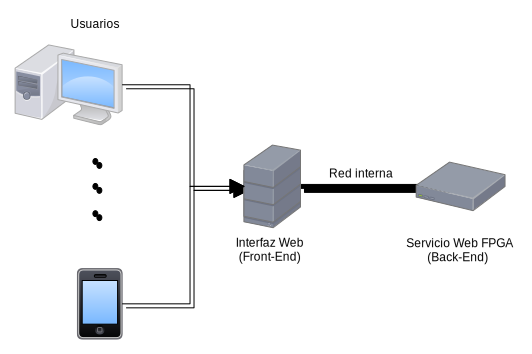
\includegraphics[width=0.7\textwidth,clip=true]{arquitectura}
  \caption{Arquitectura general de la aplicación.}
  \label{fig:arquitectura}
\end{figure}


\section{Back-End - Servicio Web FPGA\label{sec:dis:servicio_web_fpga}}

El componente \gls{back-end} se encarga de la interacción con la sonda de red (implementada en una \gls{FPGA}) y con el resto de partes involucradas en la reproducción y captura de tráfico de red.
Para ello, recibe peticiones \gls{HTTP} del \gls{front-end} (actuando en este caso como cliente), que se traducen en acciones sobre el sistema o en respuestas sobre el estado del mismo.
\begin{figure}[!htp]
  \centering
  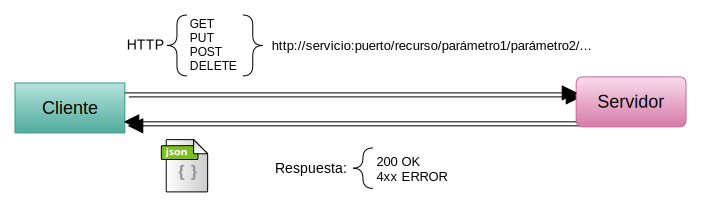
\includegraphics[width=0.95\textwidth,clip=true]{fpga_rest}
  \caption{Diagrama de flujo de un servicio \gls{REST}.}
  \label{fig:fpga_rest}
\end{figure}

La arquitectura de comunicación externa del \gls{back-end} se basa en el modelo de cliente-servidor \gls{REST} (ver Figura \ref{fig:fpga_rest}). Dentro de las directrices que marca este modelo, sólo se han considerado útiles para el problema dado un subconjunto de ellas:
\begin{itemize}
  \item El protocolo entre el cliente y el servidor debe ser sin estado: cada mensaje \gls{HTTP} tiene que contener toda la información necesaria para comprender la petición.
  \item Las operciones se aplican sobre recursos mediante llamadas a métodos \gls{HTTP}: \textit{GET} para obtener información sobre un recurso, \textit{POST}/\textit{PUT} para actualizarlos o crearlos y \textit{DELETE} para borrarlos.
  \item Cada recurso debe tener un identificador único (en este caso, una \gls{URL} única).
\end{itemize}

Se ha decidido no adoptar el resto de directrices \gls{REST} debido a que no encajaban dentro del modelo de funcionamiento de la aplicación.
Así, no se facilita el descubrimiento automático de recursos y métodos, ya que se ha considerado que no tiene sentido siendo éste un subsistema interno y no un componente público.
Por otra parte, no se permiten distintas representaciones de un mismo recurso, siendo \gls{JSON} la única representación utilizada.
No seguir estas directrices simplifica además la implementación del \gls{back-end}.

\begin{figure}[!htp]
  \centering
  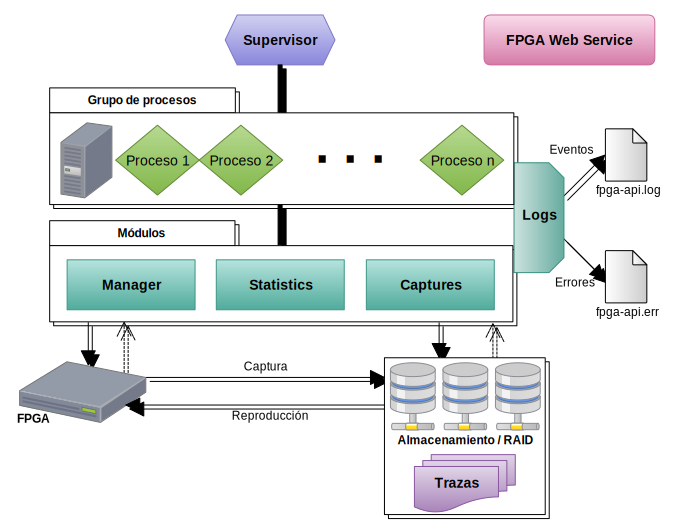
\includegraphics[width=0.95\textwidth,clip=true]{fpga}
  \caption{Arquitectura del \gls{servicioweb} \gls{FPGA}.}
  \label{fig:arquitectura_servicio}
\end{figure}

Internamente, \ref{fig:arquitectura_servicio}, 
Supervisor
1 párrafo Cluster de procesos para operaciones auxiliares, alta disponibilidad \ref{fig:arquitectura_servicio}
Logs
Módulos
Se distinguen por tanto, según su funcionalidad, tres módulos dentro del servicio web: gestión, captura y estadísticas.
\subsection{Gestión\label{ssec:dis:gestion}}

Este módulo tiene dos funciones principales: gestionar el estado de la sonda de red y gese encarga tanto de gestionar el estado de la sonda .
TODO: Gestión
  {Capturador,Reproductor}


\subsection{Capturas\label{ssec:dis:capturas}}

El módulo de capturas se encarga de todos los aspectos relacionados con las \glspl{traza} de tráfico de red.


detectar el formato interno de una \gls{traza}.

TODO: Capturas
  {Detección,Conversión,Renombrado,Borrado}


\subsection{Estadísticas\label{ssec:dis:estadisticas}}

estado, get
TODO: Estado/Estadísticas
  {Velocidad,Estado,RAID}


\section{Front-End - Interfaz web\label{sec:dis:interfaz_web}}

TODO: [Introducción] > sobre el framework, comunicación con el backend

Diseño responsive, visualmente atractiv. ventajas y diferencias vs adaptativo

Internacionalización

Introducción maquetas de las páginas principales

\subsection{Maquetas\label{ssec:dis:maquetas}}

\begin{figure}[!htp]
  \centering
  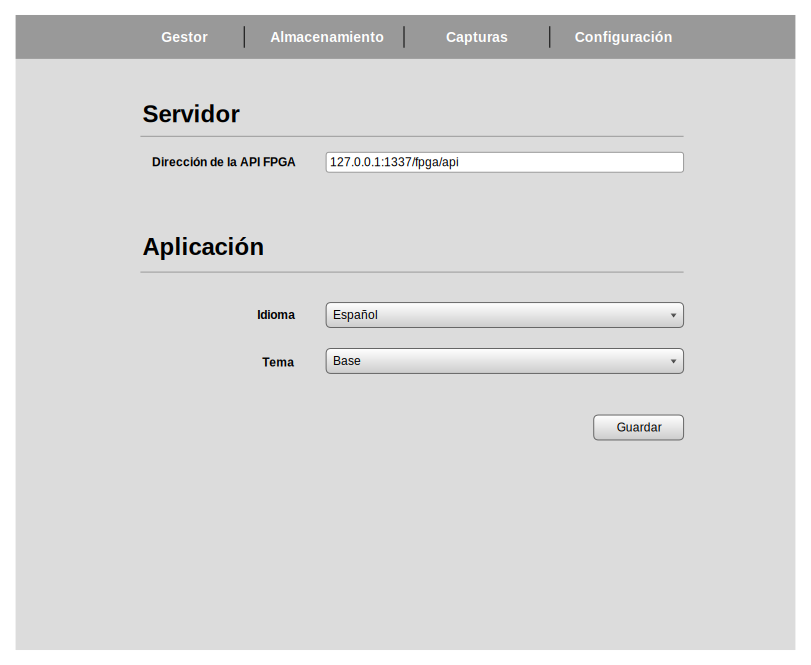
\includegraphics[width=0.95\textwidth,clip=true]{maquetas/maqueta_configuracion}
  \caption{Maqueta de la pantalla de configuración de la aplicación.}
  \label{fig:maqueta:configuracion}
\end{figure}

\begin{figure}[!htp]
  \centering
  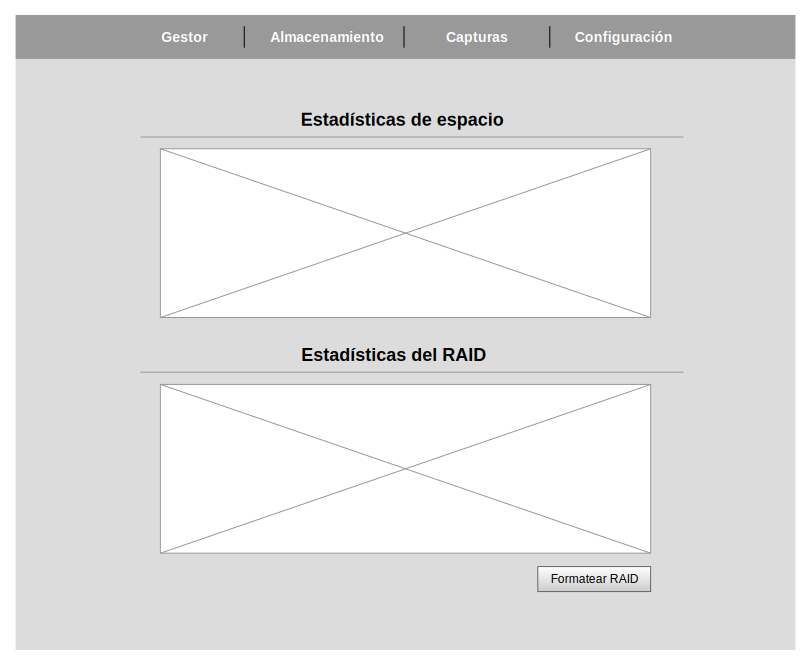
\includegraphics[width=0.95\textwidth,clip=true]{maquetas/maqueta_almacenamiento}
  \caption{Maqueta de la pantalla de almacenamiento.}
  \label{fig:maqueta:almacenamiento}
\end{figure}

\begin{figure}[!htp]
  \centering
  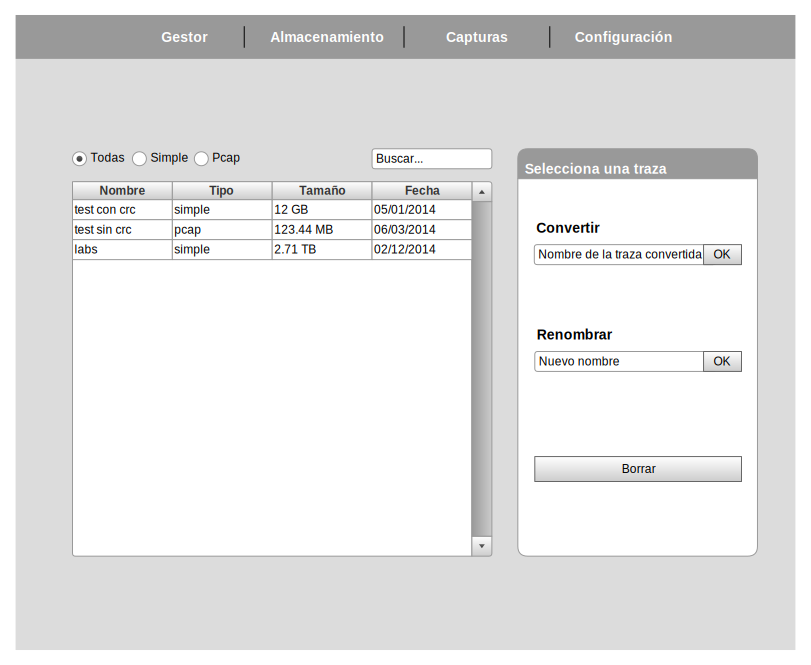
\includegraphics[width=0.95\textwidth,clip=true]{maquetas/maqueta_capturas}
  \caption{Maqueta de la pantalla de gestión de \glspl{traza}.}
  \label{fig:maqueta:capturas}
\end{figure}

\begin{figure}[!htp]
  \centering
  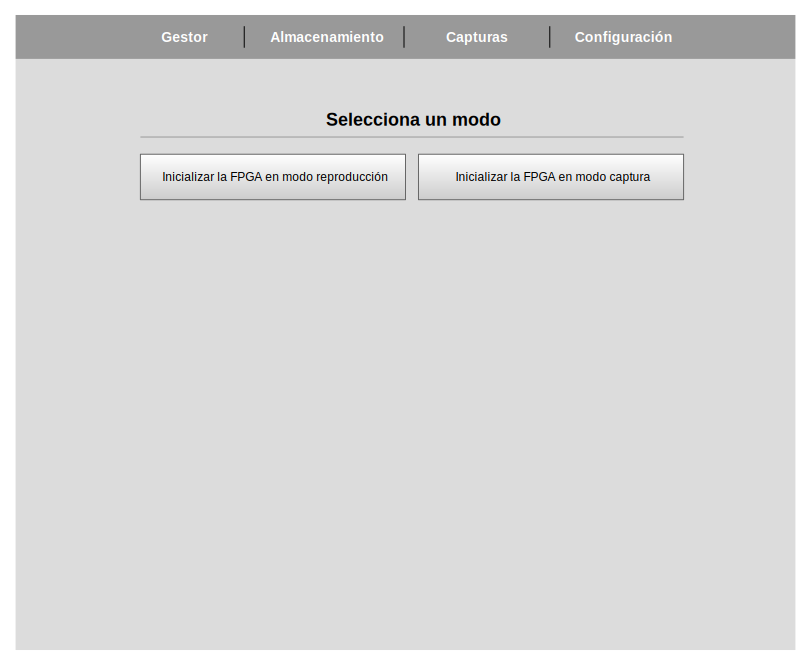
\includegraphics[width=0.95\textwidth,clip=true]{maquetas/maqueta_gestor_seleccion}
  \caption{Maqueta de la pantalla de gestión - selección de modo.}
  \label{fig:maqueta:gestor_seleccion}
\end{figure}

\begin{figure}[!htp]
  \centering
  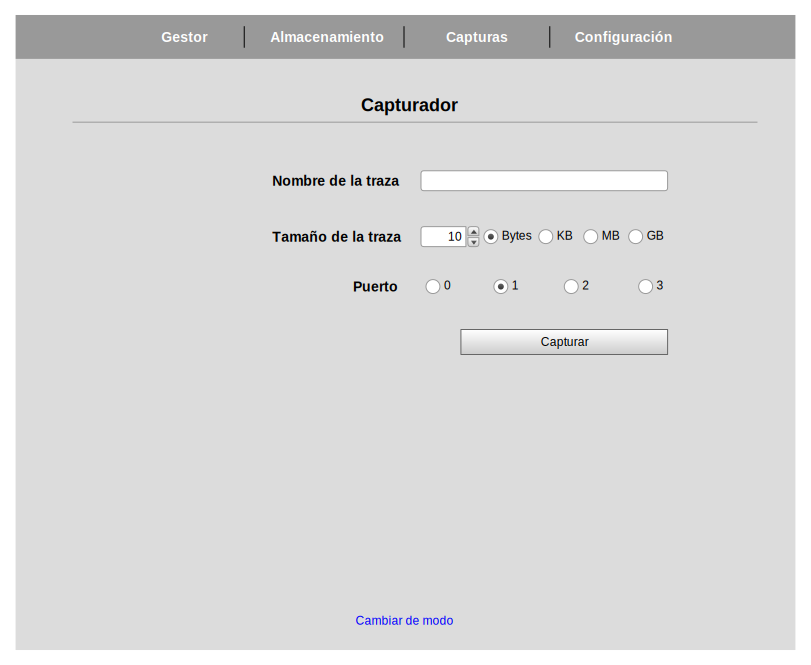
\includegraphics[width=0.95\textwidth,clip=true]{maquetas/maqueta_gestor_capturador}
  \caption{Maqueta de la pantalla de gestión - formulario para capturar.}
  \label{fig:maqueta:gestor_capturador}
\end{figure}

\begin{figure}[!htp]
  \centering
  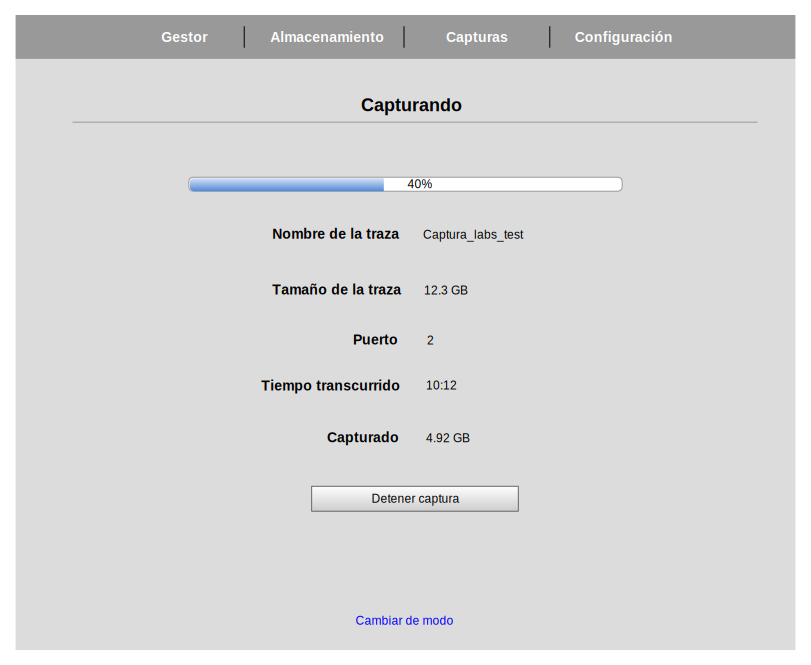
\includegraphics[width=0.95\textwidth,clip=true]{maquetas/maqueta_gestor_capturando}
  \caption{Maqueta de la pantalla de gestión - capturando.}
  \label{fig:maqueta:gestor_capturando}
\end{figure}

\begin{figure}[!htp]
  \centering
  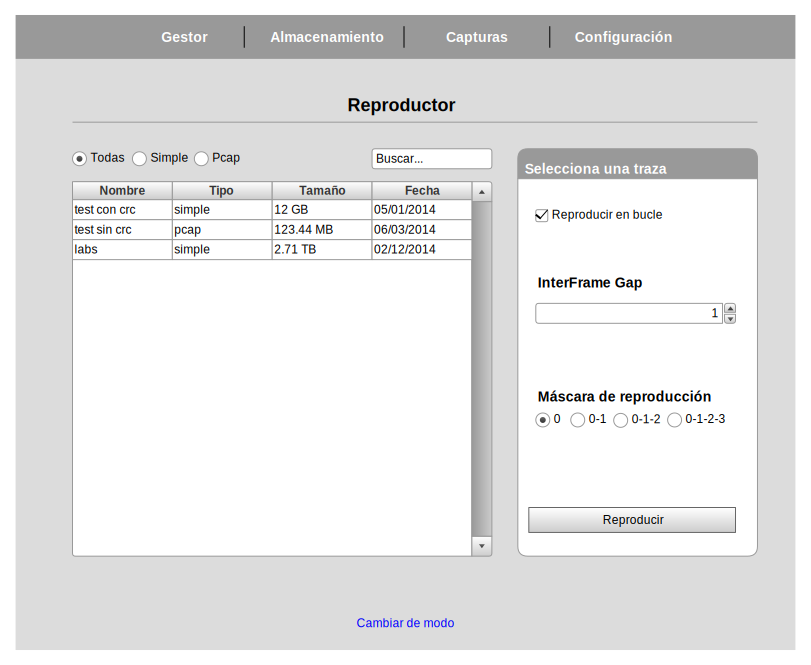
\includegraphics[width=\textwidth,clip=true]{maquetas/maqueta_gestor_reproductor}
  \caption{Maqueta de la pantalla de gestión - formulario para reproducir.}
  \label{fig:maqueta:gestor_reproductor}
\end{figure}

\begin{figure}[!htp]
  \centering
  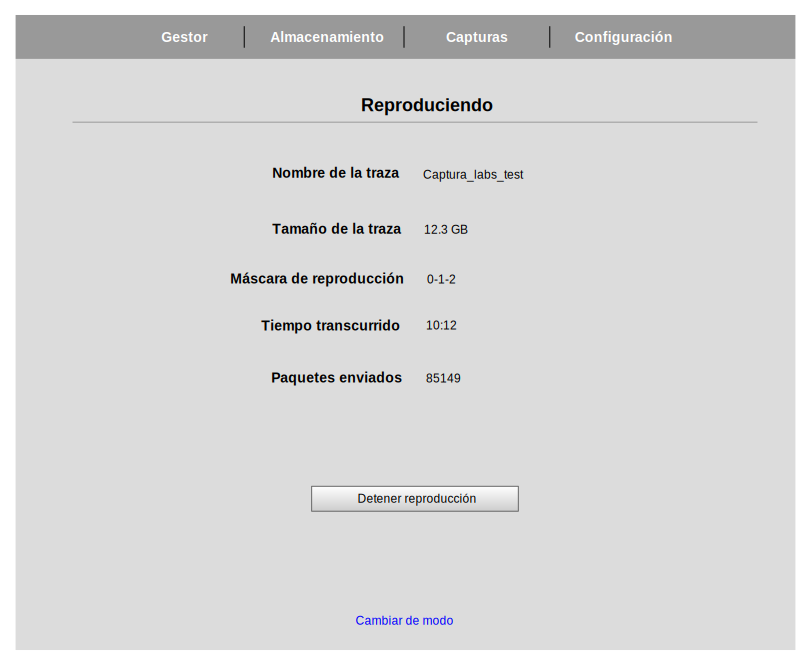
\includegraphics[width=\textwidth,clip=true]{maquetas/maqueta_gestor_reproduciendo}
  \caption{Maqueta de la pantalla de gestión - reproduciendo.}
  \label{fig:maqueta:gestor_reproduciendo}
\end{figure}
\chapter{Implementación\label{cap:implementacion}}

TODO: [Introducción]


\section{Back-End\label{sec:imp:back_end}}

TODO: Back-End
  [Introducción]
  Captura árbol de archivos
  árbol rutas?
  {io.js,express,supervisor,apiDoc,npm}
  {API ~REST,mensajes json}
  {Servicio}


\section{Front-End\label{sec:imp:front_end}}

TODO: Front-End
  [Introducción]
  Capturas diseño responsive
  Capturas árbol de archivos
  - {MVC propio,Bootstrap,jQuery,gettext,phpDocumentor}


\subsection{Internacionalización\label{ssec:imp:internacionalizacion}}

TODO: Localización


\subsection{Temas\label{ssec:imp:temas}}

TODO: Temas
\chapter{Pruebas\label{cap:pruebas}}

TODO: [Introducción]


\section{Pruebas de verificación\label{sec:pb:verificacion}}

TODO: Pruebas de verificación


\section{Pruebas de validación\label{sec:pb:validacion}}

TODO: Pruebas de validación
\chapter{Mantenimiento\label{cap:mantenimiento}}

TODO: [Introducción]
  {Open Source/GitHub Issues/Pull Requests}
\chapter{Uso de la aplicación\label{cap:uso_de_la_aplicacion}}

TODO: [Introducción]


\section{Instalación\label{sec:uso:instalacion}}

TODO: Instalación


\section{Configuración\label{sec:uso:configuracion}}

TODO: Configuración


\section{Casos de uso\label{sec:uso:casos_de_uso}}

TODO: Casos de uso
  {Apéndice Manual de Usuario}
\chapter{Conclusiones\label{cap:conclusiones}}

TODO: Conclusiones sobre el trabajo realizado
\chapter{Líneas de trabajo futuras\label{cap:lineas_de_trabajo_futuras}}

TODO: Líneas de trabajo futuras
  - Estandarización, futuras fpgas con características parecidas
  - Más idiomas
  - Más estadísticas
  - Módulo de seguridad

%
% Página en blanco
%
\cleardoublepage

%
% Bibliografía
%
\bibliography{src/bibliografia}
\addcontentsline{toc}{chapter}{Bibliografía}

%
% Apéndices
%
\appendix
\cleardoublepage
\addappheadtotoc
\appendixpage

%
% Apéndices del TFG
%
\include{src/apendice_ejemplos} % TODO: borrar
\chapter{Manual de Usuario\label{extra:manual_de_usuario}}

TODO: [Introducción]
  {Descripción detallada}
\chapter{Framework MVC propio\label{extra:framework_mvc_propio}}

TODO: [Introducción]
  {Visión global}


\section{Modelo Vista Controlador\label{extra:sec:mvc}}

TODO: Modelo Vista Controlador


\section{Manejo de dependencias\label{extra:sec:dependencias}}

TODO: Manejo de dependencias


\section{Config\label{extra:sec:config}}

TODO: Config


\section{Router\label{extra:sec:router}}

TODO: Router


\section{Logger\label{extra:sec:logger}}

TODO: Logger


\section{Conclusiones\label{extra:sec:conclusiones}}

TODO: Conclusiones
\chapter{Programación asíncrona\label{extra:programacion_asincrona}}

TODO: Programación asíncrona
\chapter{API Servicio Web FPGA\label{extra:api_servicio_web_fpga}}

TODO: API Servicio Web FPGA

{captures,manager,statistics}

% Fin del documento
\end{document}